\section{Available Hardware}
The quadcopter has been provided by Aalborg university and professor Henrik Shjøiler. This chapter has the purpose of describing the hardware. 
The hardware is tested and the results of these test will be presented. 

%removed by Niels: Firs the motor controller is outlined in the following section. 
\subsection{Motor Controller}
The quadcopter comes with four electronic speed controllers, ESCs, one for each motor. The ESCs produce an 8 kHz PWM, are rated for a 2-4 cell Li-Po battery and can handle a constant current of up to 30 A. The ESCs also has a 5.5 V, 4 A output for powering e.g. a controller board.\fxnote{source missing - \url{https://www.hobbyking.com/en_us/turnigy-multistar-30-amp-multi-rotor-brushless-esc-2-4s.html} - hobbyking took the site down - still archived by google}

\begin{figure}[H]
	\centering
	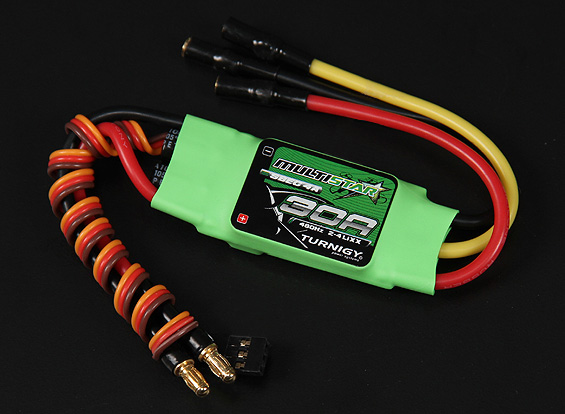
\includegraphics[scale=0.4]{figures/ESC}
	\caption{One of the four Electronic Speed Controllers mounted on the quadcopter}
	\label{fig:esc}
\end{figure}

\subsection{Motor and Propeller}
The quadrotor is equipped with four brushless outrunner motors named Turing Multistar. Bushless outrunners have in general more torque than inrunners, and can turn lager propellers, resulting in greater lift. The motors are controlled by motorcontrollers, described in another section.
The motor can be seen in \autoref{fig:Motor}.
\begin{figure}[H]
	\centering
	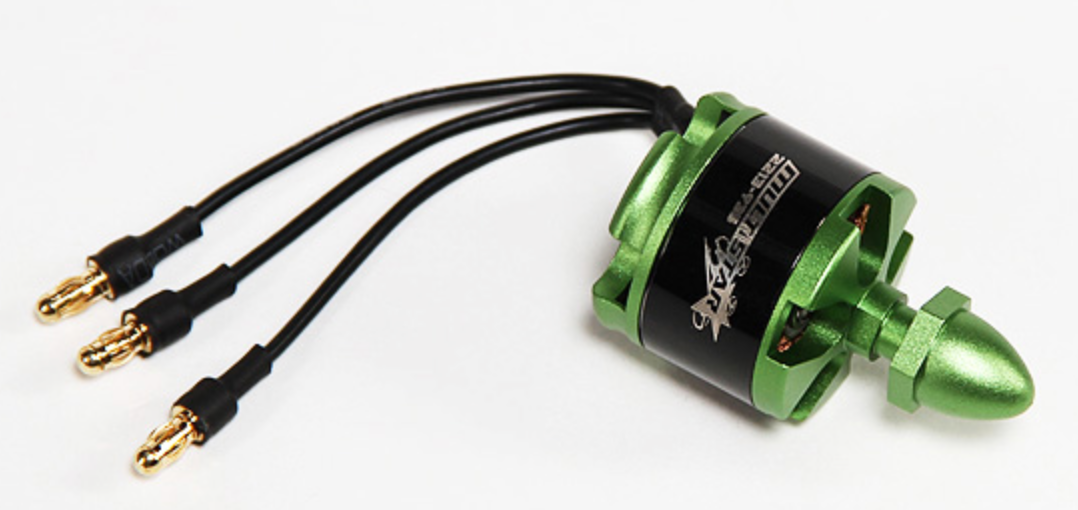
\includegraphics[scale=0.5]{figures/motor.png}
	\caption{One of the four motors mounted on the quadrotor.}
	\label{fig:Motor}
\end{figure} The propellers come with the motors. It is XX long and has a SHAPE (find proper name), see \autoref{fig:Propeller}.

\begin{figure}[H]
	\centering
	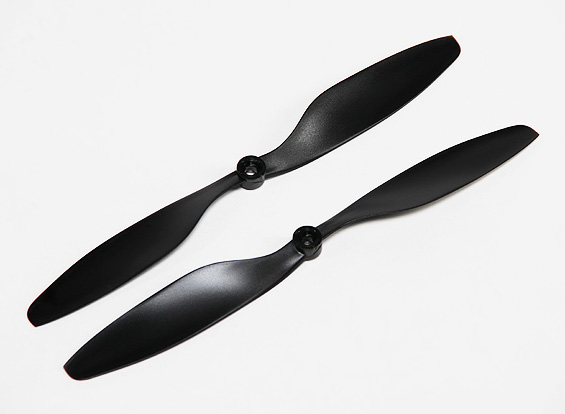
\includegraphics[scale=0.4]{figures/propeller.png}
	\caption{Two of the four propellers mounted on the quadrotor's motors.}
	\label{fig:Propeller}
\end{figure}

The relationship between PWM signal to the motor controllers and the velocity of the propeller can be seen in Figure ZZ. \fxnote{pull diagram from measurement report}

%It has been observed during tests, that the motor runs faster as it's temperature increases. This is not expected due to the increased resistance, that occurs when the coils within the motor are heated. Therefore the relationship between PWM signal and velocity is not representative for all cases. It is however deemed reasonable to neglect this variance and presume a relationship as it is derived in the measurement report, see Appendix YY. 

 
\subsection{Battery}
The battery available for the prototype, is a Zippy Flightmax battery. It weighs 141 gram, has a capacity of 1500 mAh, a voltage of 11.1 volts and a discharge current of 20 amperes.

%removed by Niels: It shall be noted, that the battery level...
The battery level drops over time, with a significance, that can not be neglected, as it has great impact on the output of the motor and therefore on the lift of the propeller. It is possible to measure the battery level while operating the quadrotor. By taking into account the battery level in the test of the PWM signal to velocity, it is possible to obtain a quadcopter having constant lift force, if this is requested\fxnote{Niels suggests: With this information and knowledge of the relationship between voltage and RPM it is possible to account for the battery level, and thereby rectify the problem. [ref to test - maybe - should the test be discussed this early?]}.

\subsection{Vicon System}
The Vicon system is a powerful tool that provides real-time position and orientation data captured with NROFCAMERAS infrared cameras. This information can be used to track objects inside a room where the system is built in.
%An example is found in Aalborg University as seen in \figref{ViconRoom}. 

%\begin{figure}[H]
%	\centering
%	\includegraphics[scale=0.5]{figures/ViconRoom}
%	\caption{Aalborg University's Vicon room.}
%	\label{ViconRoom}
%\end{figure}

To use this system, markers are attached to the object that is to be tracked. The Vicon system streams the position of the markers and the position and orientation of the object at 100 Hz for a computer to read them. The data can be received by using an SDK plugin for MATLAB. In this way, data can be operated in the MATLAB environment, making it easier to obtain variable derivatives like velocities or accelerations.

The user interface of the Vicon system is shown in \autoref{fig:ViconTracker}. 
\begin{figure}[H]
	\centering
	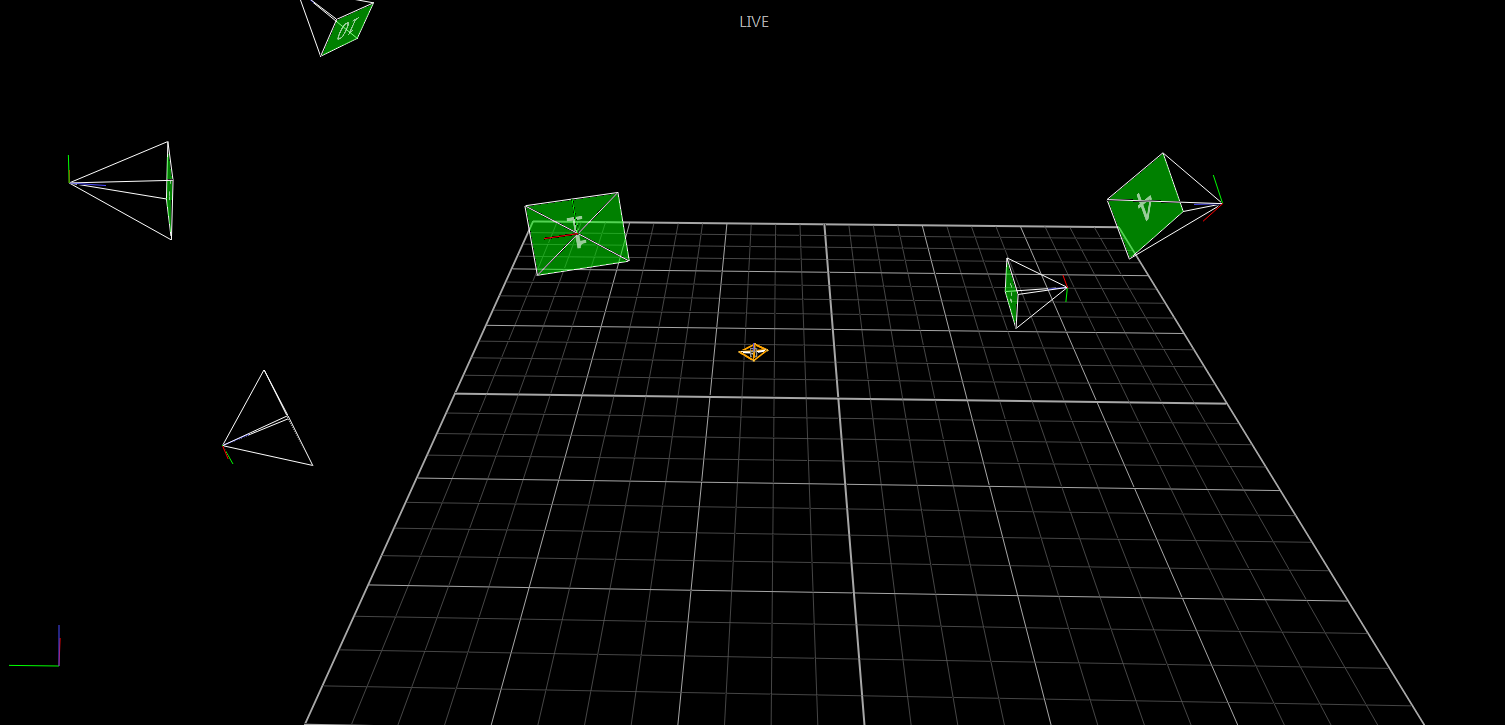
\includegraphics[scale=0.27]{figures/ViconTracker}
	\caption{User interface of the Vicon System, the Vicon Tracker. An object has been created from the markers placed on the drone.}
	\label{fig:ViconTracker}
\end{figure}
It is called Vicon Tracker and it allows the creation of objects by grouping markers present in the room. It also allows to change the center of gravity of the created objects and rotate the inertial and body reference frames to any desired orientation.